\documentclass[journal,twoside,web]{ieeecolor}
\usepackage{jsen}
\usepackage{cite}
\usepackage{amsmath,amssymb,amsfonts}
\usepackage{algorithmic}
\usepackage{graphicx}
\usepackage{textcomp}
\usepackage{wrapfig}
\usepackage{siunitx}
\def\BibTeX{{\rm B\kern-.05em{\sc i\kern-.025em b}\kern-.08em
    T\kern-.1667em\lower.7ex\hbox{E}\kern-.125emX}}
\markboth{\journalname, Advance telecommunication design specification 2023}
{Author \MakeLowercase{\textit{et al.}}: Optical multiplexer/demultiplexer specification document (November 2023)}
\definecolor{abstractbg}{rgb}{0.89804,0.94510,0.83137}
\setlength{\fboxrule}{0pt}
\setlength{\fboxsep}{0pt}
\begin{document}
\title{Optical multiplexer/demultiplexer specification document (November 2023)}
\author{Daniël van Langeveld, \IEEEmembership{3875393}, Fer Clerkx, \IEEEmembership{4331052} (Group 6)
}

\IEEEtitleabstractindextext{%
\fcolorbox{abstractbg}{abstractbg}{%
\begin{minipage}{\textwidth}%
\begin{wrapfigure}[10]{r}{3in}%
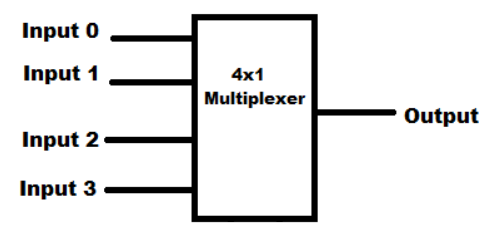
\includegraphics[width=2.5in]{images/mux.png}%
\end{wrapfigure}%
\begin{abstract}
This document describes the system which will be designed for S7 advanced telecommunications.
The goal of this assignment is to theoretically design and simulate the requirements and functions
of an optical multiplexer. This design will not be build in practice because of certain limitations
of the fontys engineering faculty. Specifically, it describes a multiplexer/demultiplexer which can 
be used to transmit more than one instance of data at the same time. This can be done by adding 
wave forms together without any manipulation or by first converting it to an electronic signal, 
then multiplexing, and finally sending out the final signal as light again. Finally, this document 
also describes the characteristics of modern multiplexing methods
\end{abstract}

\begin{IEEEkeywords}
Demultiplexer, Fontys, Multiplexer, Optical signal 
\end{IEEEkeywords}
\end{minipage}}}

\maketitle

\section{Introduction}
\label{sec:introduction}
\IEEEPARstart {T}{his} document describes the specifications of the optical 
mulitplexer/demultiplexer Group 6 of advanced telecommunications will simulate 
reading a paper or PDF version of this document, please download the 
electronic file, trans\_jour.tex, from the IEEE Web site at \underline
{http://www.ieee.org/authortools/trans\_jour.tex} so you can use it to prepare your manuscript. If 
you would prefer to use LaTeX, download IEEE's LaTeX style and sample files 
from the same Web page. You can also explore using the Overleaf editor at 
\underline
{https://www.overleaf.com/blog/278-how-to-use-overleaf-with-}\discretionary{}{}{}\underline
{ieee-collabratec-your-quick-guide-to-getting-started\#.}\discretionary{}{}{}\underline{xsVp6tpPkrKM9}

If your paper is intended for a conference, please contact your conference 
editor concerning acceptable word processor formats for your particular 
conference. 

IEEE will do the final formatting of your paper. If your paper is intended 
for a conference, please observe the conference page limits. 

\subsection{Abbreviations and Acronyms}
Define abbreviations and acronyms the first time they are used in the text, 
even after they have already been defined in the abstract. Abbreviations 
such as IEEE, SI, ac, and dc do not have to be defined. Abbreviations that 
incorporate periods should not have spaces: write ``C.N.R.S.,'' not ``C. N. 
R. S.'' Do not use abbreviations in the title unless they are unavoidable 
(for example, ``IEEE'' in the title of this article).

\subsection{Other Recommendations}
Use one space after periods and colons. Hyphenate complex modifiers: 
``zero-field-cooled magnetization.'' Avoid dangling participles, such as, 
``Using \eqref{eq}, the potential was calculated.'' [It is not clear who or what 
used \eqref{eq}.] Write instead, ``The potential was calculated by using \eqref{eq},'' or 
``Using \eqref{eq}, we calculated the potential.''

Use a zero before decimal points: ``0.25,'' not ``.25.'' Use 
``cm$^{3}$,'' not ``cc.'' Indicate sample dimensions as ``0.1 cm 
$\times $ 0.2 cm,'' not ``0.1 $\times $ 0.2 cm$^{2}$.'' The 
abbreviation for ``seconds'' is ``s,'' not ``sec.'' Use 
``Wb/m$^{2}$'' or ``webers per square meter,'' not 
``webers/m$^{2}$.'' When expressing a range of values, write ``7 to 
9'' or ``7--9,'' not ``7$\sim $9.''

A parenthetical statement at the end of a sentence is punctuated outside of 
the closing parenthesis (like this). (A parenthetical sentence is punctuated 
within the parentheses.) In American English, periods and commas are within 
quotation marks, like ``this period.'' Other punctuation is ``outside''! 
Avoid contractions; for example, write ``do not'' instead of ``don't.'' The 
serial comma is preferred: ``A, B, and C'' instead of ``A, B and C.''

If you wish, you may write in the first person singular or plural and use 
the active voice (``I observed that $\ldots$'' or ``We observed that $\ldots$'' 
instead of ``It was observed that $\ldots$''). Remember to check spelling. If 
your native language is not English, please get a native English-speaking 
colleague to carefully proofread your paper.

Try not to use too many typefaces in the same article. You're writing
scholarly papers, not ransom notes. Also please remember that MathJax
can't handle really weird typefaces.

\subsection{Equations}
Number equations consecutively with equation numbers in parentheses flush 
with the right margin, as in \eqref{eq}. To make your equations more 
compact, you may use the solidus (~/~), the exp function, or appropriate 
exponents. Use parentheses to avoid ambiguities in denominators. Punctuate 
equations when they are part of a sentence, as in
\begin{equation}E=mc^2.\label{eq}\end{equation}

Be sure that the symbols in your equation have been defined before the 
equation appears or immediately following. Italicize symbols ($T$ might refer 
to temperature, but T is the unit tesla). Refer to ``\eqref{eq},'' not ``Eq. \eqref{eq}'' 
or ``equation \eqref{eq},'' except at the beginning of a sentence: ``Equation \eqref{eq} 
is $\ldots$ .''

\subsection{\LaTeX-Specific Advice}

Please use ``soft'' (e.g., \verb|\eqref{Eq}|) cross references instead
of ``hard'' references (e.g., \verb|(1)|). That will make it possible
to combine sections, add equations, or change the order of figures or
citations without having to go through the file line by line.

Please don't use the \verb|{eqnarray}| equation environment. Use
\verb|{align}| or \verb|{IEEEeqnarray}| instead. The \verb|{eqnarray}|
environment leaves unsightly spaces around relation symbols.

Please note that the \verb|{subequations}| environment in {\LaTeX}
will increment the main equation counter even when there are no
equation numbers displayed. If you forget that, you might write an
article in which the equation numbers skip from (17) to (20), causing
the copy editors to wonder if you've discovered a new method of
counting.

{\BibTeX} does not work by magic. It doesn't get the bibliographic
data from thin air but from .bib files. If you use {\BibTeX} to produce a
bibliography you must send the .bib files. 

{\LaTeX} can't read your mind. If you assign the same label to a
subsubsection and a table, you might find that Table I has been cross
referenced as Table IV-B3. 

{\LaTeX} does not have precognitive abilities. If you put a
\verb|\label| command before the command that updates the counter it's
supposed to be using, the label will pick up the last counter to be
cross referenced instead. In particular, a \verb|\label| command
should not go before the caption of a figure or a table.

Do not use \verb|\nonumber| inside the \verb|{array}| environment. It
will not stop equation numbers inside \verb|{array}| (there won't be
any anyway) and it might stop a wanted equation number in the
surrounding equation.

If you are submitting your paper to a colorized journal, you can use
the following two lines at the start of the article to ensure its
appearance resembles the final copy:

\smallskip\noindent
\begin{small}
\begin{tabular}{l}
\verb+\+\texttt{documentclass[journal,twoside,web]\{ieeecolor\}}\\
\verb+\+\texttt{usepackage\{\textit{Journal\_Name}\}}
\end{tabular}
\end{small}
\section{background}
\label{sec:background}

The first step in designing a system is to explore what methods are currently 
available. A few of the main ways optical signals are currently multiplexed are: time-division 
multiplexing, frequency/wavelength-division multiplexing and spatial multiplexing.

\subsection{Time-division multiplexing}
Time-division multiplexing makes use of specific time-windows in which it sends what data.
An example of this would be that the multiplexer sends data from one source for \qty{1}{\ms}, 
after which it sends the data from the next source for \qty{1}{\ms} and so on, untill it comes 
back to the data from the first source and it keeps repeating this cycle. Possible downsides of
this method are that both sides need synchronized clocks to acknowledgde when the data from 
each source is sent and the possibility of requiring a larger cache to store the data waiting 
for its timeslot to be sent

\subsection{Spatial multiplexing}
Spatial multiplexing keeps the data from each source physically separate from other data sent 
at the same time. Ways of achieving for optical communication include multifibre cables, 
multi-modal fibres and waveguides. Downsides of this technique mostly come down to high requirements 
for the transmitters, receivers and fibres themselves. Where time-division multiplexing is able to be 
sent through almost any optical fibre cable, spatial multiplexed signals set strict requirements, like 
multi-core cables which are thicker, special and experimental crystals at the transmitter, or optical cables 
without defects or minimal bends between transmitter and receiver.

\subsection{Wavelength-division multiplexing}
Wavelength-division multiplexing or WDM uses lasers of differing wavelengths between \qty{1270}{\nm} and 
\qty{1610}{\nm} to send multiple signals at once through an optical cable. If the frequencies are spaced 
correctly, with some room in between, they should not interfere with eachother. Usually this goes correctly, 
but since there are no physical or temporal divisions between the signals, this method does have one of the 
highest chances of destructive interference among the previously mentioned methods. If the channel size is large 
enough, there is no problem. In practice the channel is about \qty{20}{\nm} in the least dense method (CWDM), 
but other techniques(DWDM) exist which allow more data to be send on smaller channels. A plus side of this method 
is that the requirements of the fibre optic cable are lower than for most spatial multiplexing methods.

\subsection{Optical Add/Drop Multiplexer}
A specific device which makes use of the functionalities of WDMs is the Optical Add/Drop Multiplexer(OADM). This 
device demultiplexes the signal, is able to remove one or more signals, and add some more signals to the stream. 
At the output of the OADM, the signal is multiplexed again and send on to the next node in the optic fibre cable.
Dependent on the specific construction of the Multiplexer, either O/E or straight optical, some devices are able 
to amplify the signal before sending it out again.

\subsection{Attenuation loss}
As mentioned in the OADM subsection, signals can be amplified by some devices. This is necessarry since the 
signal can lose its strength. The two main ways signals lose their strength is either loss by absorbtion 
or loss by scattering. The first loss is caused by the fact that the transport medium, usually a kind of glass, 
absorbs a part of the light. This kind of loss is usually expressed in dB/km, and preferably is as low as possible, 
especially for long distance communication. The second kind of loss is caused by bends in the cable. Light waves, 
prefer to travel in straight lines and when a bend occurs, some of the light will try to still go straight. This 
causes losses usually expressed in dB loss over a specific bend radius. 

\section{Specifications}
\label{sec:specifications}
This chapter lays out the specification used to design the wavelength division modulation (WDM) system. See table \ref{table:specs1} and table \ref{table:specs2}.

\begin{table}[!ht]
	\centering
	\cite{noauthor_gofoton_nodate}
	\begin{tabular} {|l|c|}
		\hline
		\multicolumn{1}{|c|}{\textbf{Parameter}} & \textbf{Unit} \\ \hline\hline
		Operating Wavelength & \unit{\nm} \\ \hline
		Channel spacing & \unit{\GHz} \\ \hline
		Center Wavelength & \unit{\nm} \\ \hline
		Upgrade Port Wavelength Range (Option) & \unit{\nm} \\ \hline
		Express Port Wavelength Range (Option) & \unit{\nm} \\ \hline
		Passband Band Width & \unit{\nm} \\ \hline
		DWDM port Insertion Loss & \unit{\dB} \\ \hline
		Express Port Wavelength (option) & \unit{\dB} \\ \hline
		Upgrade Port Insertion Loss (option) & \unit{\dB} \\ \hline
		Passband Ripple & \unit{\dB} \\ \hline
		Adjacent Channel Isolation & \unit{\dB} \\ \hline
		Non-Adjacent Channel Isolation & \unit{\dB} \\ \hline
		Upgrade Port Isolation & \\ \hline
		Express port isolation & \\ \hline
		Polarization Dependent Loss & \unit{\dB} \\ \hline
		Optical Return Loss & \unit{\dB} \\ \hline
		Directivity & \unit{\dB} \\ \hline
		Optical Power Handling & \unit{\mW} \\ \hline
		Operating Temperature Range & \unit{\degreeCelsius} \\ \hline
		Storage Temperature Range & \unit{\degreeCelsius} \\ \hline
		Fiber Type & - \\ \hline
		Fiber Jacket & - \\ \hline
		Package Size & \unit{\mm} \\ \hline
		Number of Channels & - \\ \hline
		Accessibility & - \\ \hline
	\end{tabular}
	\caption{List of specifications GOFOTON DWDM}
	\label{table:specs1}
\end{table}

\begin{table}[!ht]
	\centering
	\cite{noauthor_4ch_nodate}
	\begin{tabular} {|l|c|}
		\hline
		\multicolumn{1}{|c|}{\textbf{Parameter}} & \textbf{Unit} \\ \hline\hline
		Center Wavelength & \unit{\nm} \\ \hline
		Channel Spacing & \unit{\nm} \\ \hline
		Channel Passband & \unit{\nm} \\ \hline
		Insertion Loss (Passband) & \unit{\dB} \\ \hline
		Technology & - \\ \hline
		Passband Ripple & \unit{\dB} \\ \hline
		Directivity & \unit{\dB} \\ \hline
		Return Loss & \unit{\dB} \\ \hline
		PDL & \unit{\dB} \\ \hline
		PMD & \unit{\ps} \\ \hline
		Power Handling & \unit{\mW} \\ \hline
		Operating Temperature & \unit{\degreeCelsius} \\ \hline
		Storage Temperature & \unit{\degreeCelsius} \\ \hline
		Connector Type & - \\ \hline
		Dimensions (H x W x D) & \unit{\mm} \\ \hline
	\end{tabular}
	\caption{List of specifications FS CWDM}
	\label{table:specs2}
\end{table}

% \begin{itemize}
%  \item The inputs and outputs of the system are optical.
%  \item The signals will not be converted to the electrical domain at any stage (no O/E/O). 
%  \item Single mode fibre will be used.
%  \item 4 channels are used.
%  \item TX and RX signals use a common fiber.
%  \item The system can perform both MUX and DEMUX operations.
%  \item The channel wavelengths are spaced \qty{20}{\nm} apart.
% \end{itemize}

% The inputs and outputs of the system are all optical, as transponders fall outside the 
% scope of the system. By also keeping the signals in the optical domain, the mux and demux 
% operation has to be performed in the optical domain. Single mode fiber will be used, 
% meaning it is up to the user to make sure that each input is matched to the correct channel. 
% Single mode fiber was chosen such that modal dispersion doesn't have to be accounted for. 
% Lastly, individual channels will be spaced \qty{20}{\nm} apart, making it a CWDM system.

% From the above requirements a MUX/DEMUX system will be designed. An overiew of the of these 
% systems in a link is given in figure \ref{fig:link_overview}.

% \begin{figure}[ht]
%     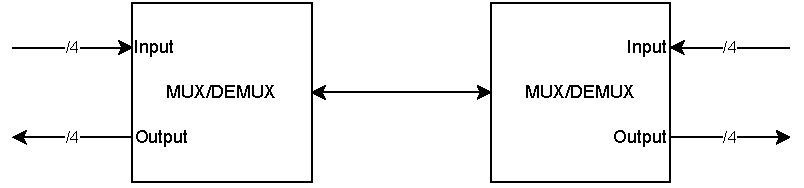
\includegraphics[width=\linewidth]{images/link_overview.pdf}
%     \caption{Overview of MUX/DEMUX link}
%     \label{fig:link_overview}
% \end{figure}

\appendices

% Appendixes, if needed, appear before the acknowledgment.

\end{document}